% !TeX spellcheck = en_GB
\chapter{Experimental Setup}

\begin{comment}
	* TODO
\end{comment}


\section{Simulation Environment}

Regarding the established methodology for enabling the implementation of the proposed solution, the \textit{grid2Op} framework \cite{rtefranceGrid2OpDocumentation} will be used for modelling the sequential decision-making process on simulated power distribution grid. \textit{grid2Op} is designed by RTE (\textit{Réseau de Transport d'Électricité}), the electricity transmission system operator of France, and is equipped with a variety of pre-defined scenarios used in coding competitions and based on real-world data \cite{rtefranceGrid2OpDocumentation}. This platform focuses on easing the job using the grid topology to control the power flows and also allowing for it to be reconfigured in real-time \cite{rtefranceGrid2OpDocumentation}. Additionally, enables to graphically plot the current observable state of the grid, as portrayed in figure \ref{fig:grid2op-graph}. Apart from graph topology, \textit{grid2op} also enables the manipulation of:

\begin{itemize}
	\item the \textbf{voltages} by manipulating the set-point value of the generators;
	\item the \textbf{active generation} by mapping the received observations to optimal sequences of dispatch actions \cite{rtefranceGrid2OpDocumentation}
\end{itemize}

This framework is compatible with the \textit{Gymnasium} framework \cite{faramafoundationGymnasiumDocumentation}, a widely used toolkit for developing \ac{RL} algorithms, which will also will be used in this work together with the Grid2Op simulation environment. 

\begin{figure}
	\centering
	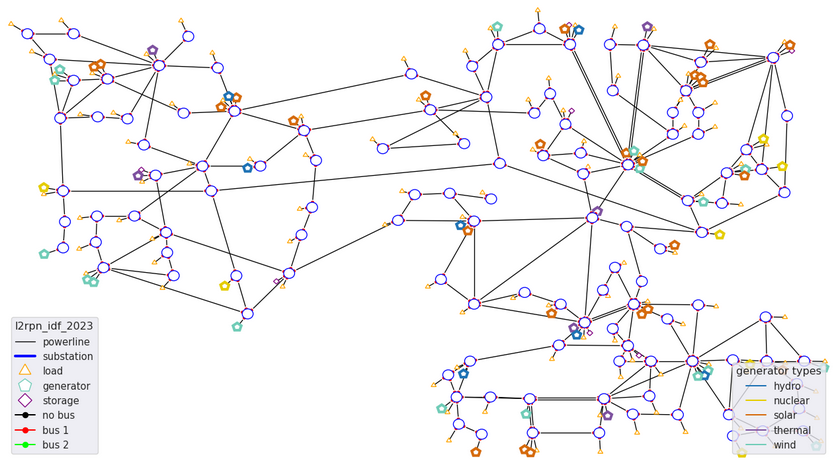
\includegraphics[width=0.85\linewidth]{./figures/grid2op-graph.png}
	\caption{Grid2Op \textit{l2rpn\_idf\_2023} 118-bus test case \cite{rtefranceGrid2OpDocumentation}}
	\label{fig:grid2op-graph}
\end{figure}

This platform focuses on describing the power distribution grids by modelling the following objects:
\begin{itemize}
	\item \textbf{Buses} are the fundamental objects of the power grid, representing nodes where power sources, loads and other elements are connected\cite{rtefranceGrid2OpDocumentation}.
	
	\item \textbf{Powerlines} represent edges in the power grid and connect the different buses together. They represent the physical transmission and distribution lines and allow power to flow from one part of the grid to another \cite{rtefranceGrid2OpDocumentation}.
	
	\item \textbf{Generators} are critical grid elements connected to buses whose main role is to produce power and maintain grid stability by balancing the energy supply and demand. They can be Conventional Thermal Generators, Wind Turbines or Photovoltaic Cells \cite{rtefranceGrid2OpDocumentation}.
	
	\item \textbf{Loads} consume power from the grid, simulating electricity use. They're also associated to an individual bus \cite{rtefranceGrid2OpDocumentation}.
	
	\item \textbf{Storage Units} can act as both consumers and producers. They're able to retain energy from the power grid when production surpasses demand for later injecting back power when convenient. Storage units are bound by a maximum energy storage capacity \cite{rtefranceGrid2OpDocumentation}.
\end{itemize}


Beyond \textit{grid2op} to build and run the test cases and \textit{gymnasium} as the RL framework, this project will use \textit{PyTorch} \cite{pytorchPyTorch} with \textit{PyTorch Geometric} \cite{pygteamPyGPytorch_geometric} library for developing the \ac{GNN} because of its extensive list of available implemented models. The different combinations of algorithms will be applied to a set of modified scenarios that fulfil the settled requirements. For Deep Reinforcement Learning algorithms, solutions with plain \ac{SAC}, \ac{DDPG} and \ac{PPO} approaches and combined with the \ac{GCN}, \ac{GAT} and \ac{GIN} architectures.  \par
Concerning result analysis, it's also important to point out the use of quantitative methods for evaluating the different implemented models, a topic that is further explored in the following section \ref{sec:eval-methods}.

\section{Scenarios}

\begin{table}[H] 
	\centering
	\caption{Test Case Sizes}
	\begin{tabular}{|P{2cm}|P{3.5cm}|P{3.5cm}|  }
		\hline
		& \textbf{l2rpn\_icaps\_2021} & \textbf{l2rpn\_idf\_2023} \\
		\hline
		\textbf{Buses} & 36 & 118 \\
		\hline
		\textbf{Powerlines} & 59  & 186  \\
		\hline
		\textbf{Generators} & 22 & 62  \\
		\hline
		\textbf{Loads} & 37 & 99 \\
		\hline
	\end{tabular}
	\label{tab:test-case}
\end{table}

This work will use the pre-defined \textit{grid2op} \textit{l2rpn\_icaps\_2021} and \textit{l2rpn\_idf\_2023} test environments, a modified case studies based on the original IEEE 118-bus system test case \cite{christiePowerSystemsTesta} of 36 and 118 buses, respectively. The first test case is a subset of the original 118-bus system with 50 years worth of data divided into independent \footnote{non-consecutive} weekly scenarios, while in the second case the system was modified to accommodate the \textit{possible energy mix} of France in 2035, containing 16 years of data \cite{rtefranceGrid2OpDocumentation}. The scenarios document the loads and productions at each time step, the grid layout (for display purposes), generator and \ac{ESS} characteristics \cite{rtefranceGrid2OpDocumentation} for a weekly episode, the sizes of test cases can be further observed in table \ref{tab:test-case}. In addition, the test cases data will be modified to reflect the defined requirements of this work. \par

\section{Experiments}

\subsection{GRL}

\subsection{DRL vs. GRL}

\subsection{Scalability}

\subsection{Adaptability}


